\documentclass[aspectratio=169,11pt]{beamer}
\usetheme{Madrid}
\usecolortheme{default}
\setbeamertemplate{navigation symbols}{}
\setbeamertemplate{footline}[frame number]
\setbeamertemplate{itemize items}[circle]
\usepackage[T1]{fontenc}
\usepackage[utf8]{inputenc}
\usepackage{lmodern}
\usepackage{graphicx}
\usepackage{booktabs}
\usepackage{array}
\usepackage{xcolor}
\usepackage{ragged2e}
\graphicspath{{plots/}}

\definecolor{accent}{RGB}{25,72,140}
\definecolor{muted}{RGB}{85,85,85}

\setbeamercolor{title}{fg=accent}
\setbeamercolor{frametitle}{fg=accent}
\setbeamercolor{structure}{fg=accent}
\setbeamercolor{normal text}{fg=black,bg=white}

\title{Strategic Allocation Scenario Framework}
\subtitle{Long-Horizon Benchmark and Regime Interpretation}
\author{XOPTPOE}
\date{}

\begin{document}

\begin{frame}
  \titlepage
\end{frame}

\begin{frame}{What We Are Doing}
\begin{itemize}
  \item We build a long-horizon strategic allocation framework across 9 investable sleeves.
  \item The system forms 5-year and 10-year return views and maps them into portfolio decisions.
  \item The main interpretation object is the robust 5-year benchmark portfolio.
  \item The key question is: what macro-financial regimes justify stronger, weaker, broader, or more defensive benchmark outcomes?
\end{itemize}
\vspace{0.6em}
{\small\color{muted}This is a strategic allocation framework, not a short-term trading system.}
\end{frame}

\begin{frame}{Investment Universe and Horizon}
\begin{columns}[T,totalwidth=\textwidth]
\column{0.52\textwidth}
\textbf{Asset classes}
\begin{itemize}
  \item US Equities
  \item Euro Area Equities
  \item Japan Equities
  \item China Equities
  \item Emerging Market Equities
  \item US Treasuries 7--10Y
  \item Investment Grade Credit
  \item Gold
  \item US REITs
\end{itemize}

\column{0.48\textwidth}
\textbf{Core framing}
\begin{itemize}
  \item Main strategic horizon: 5 years
  \item Secondary reference horizon: 10 years
  \item Active benchmark: robust 5-year benchmark portfolio
  \item Scenario analysis is centered on this single benchmark object
\end{itemize}
\end{columns}
\end{frame}

\begin{frame}{The Benchmark Behaves Credibly}
\begin{columns}[T,totalwidth=\textwidth]
\column{0.43\textwidth}
\begin{itemize}
  \item The benchmark beats equal weight on a risk-adjusted basis in the walk-forward illustration.
  \item Portfolio behavior is interpretable rather than random or unstable.
  \item This gives a credible object to probe with scenarios.
\end{itemize}
\vspace{0.8em}
{\small\color{muted}Supporting diagnostics are long-horizon decision diagnostics rather than a claim of a clean tradable monthly backtest.}

\column{0.57\textwidth}
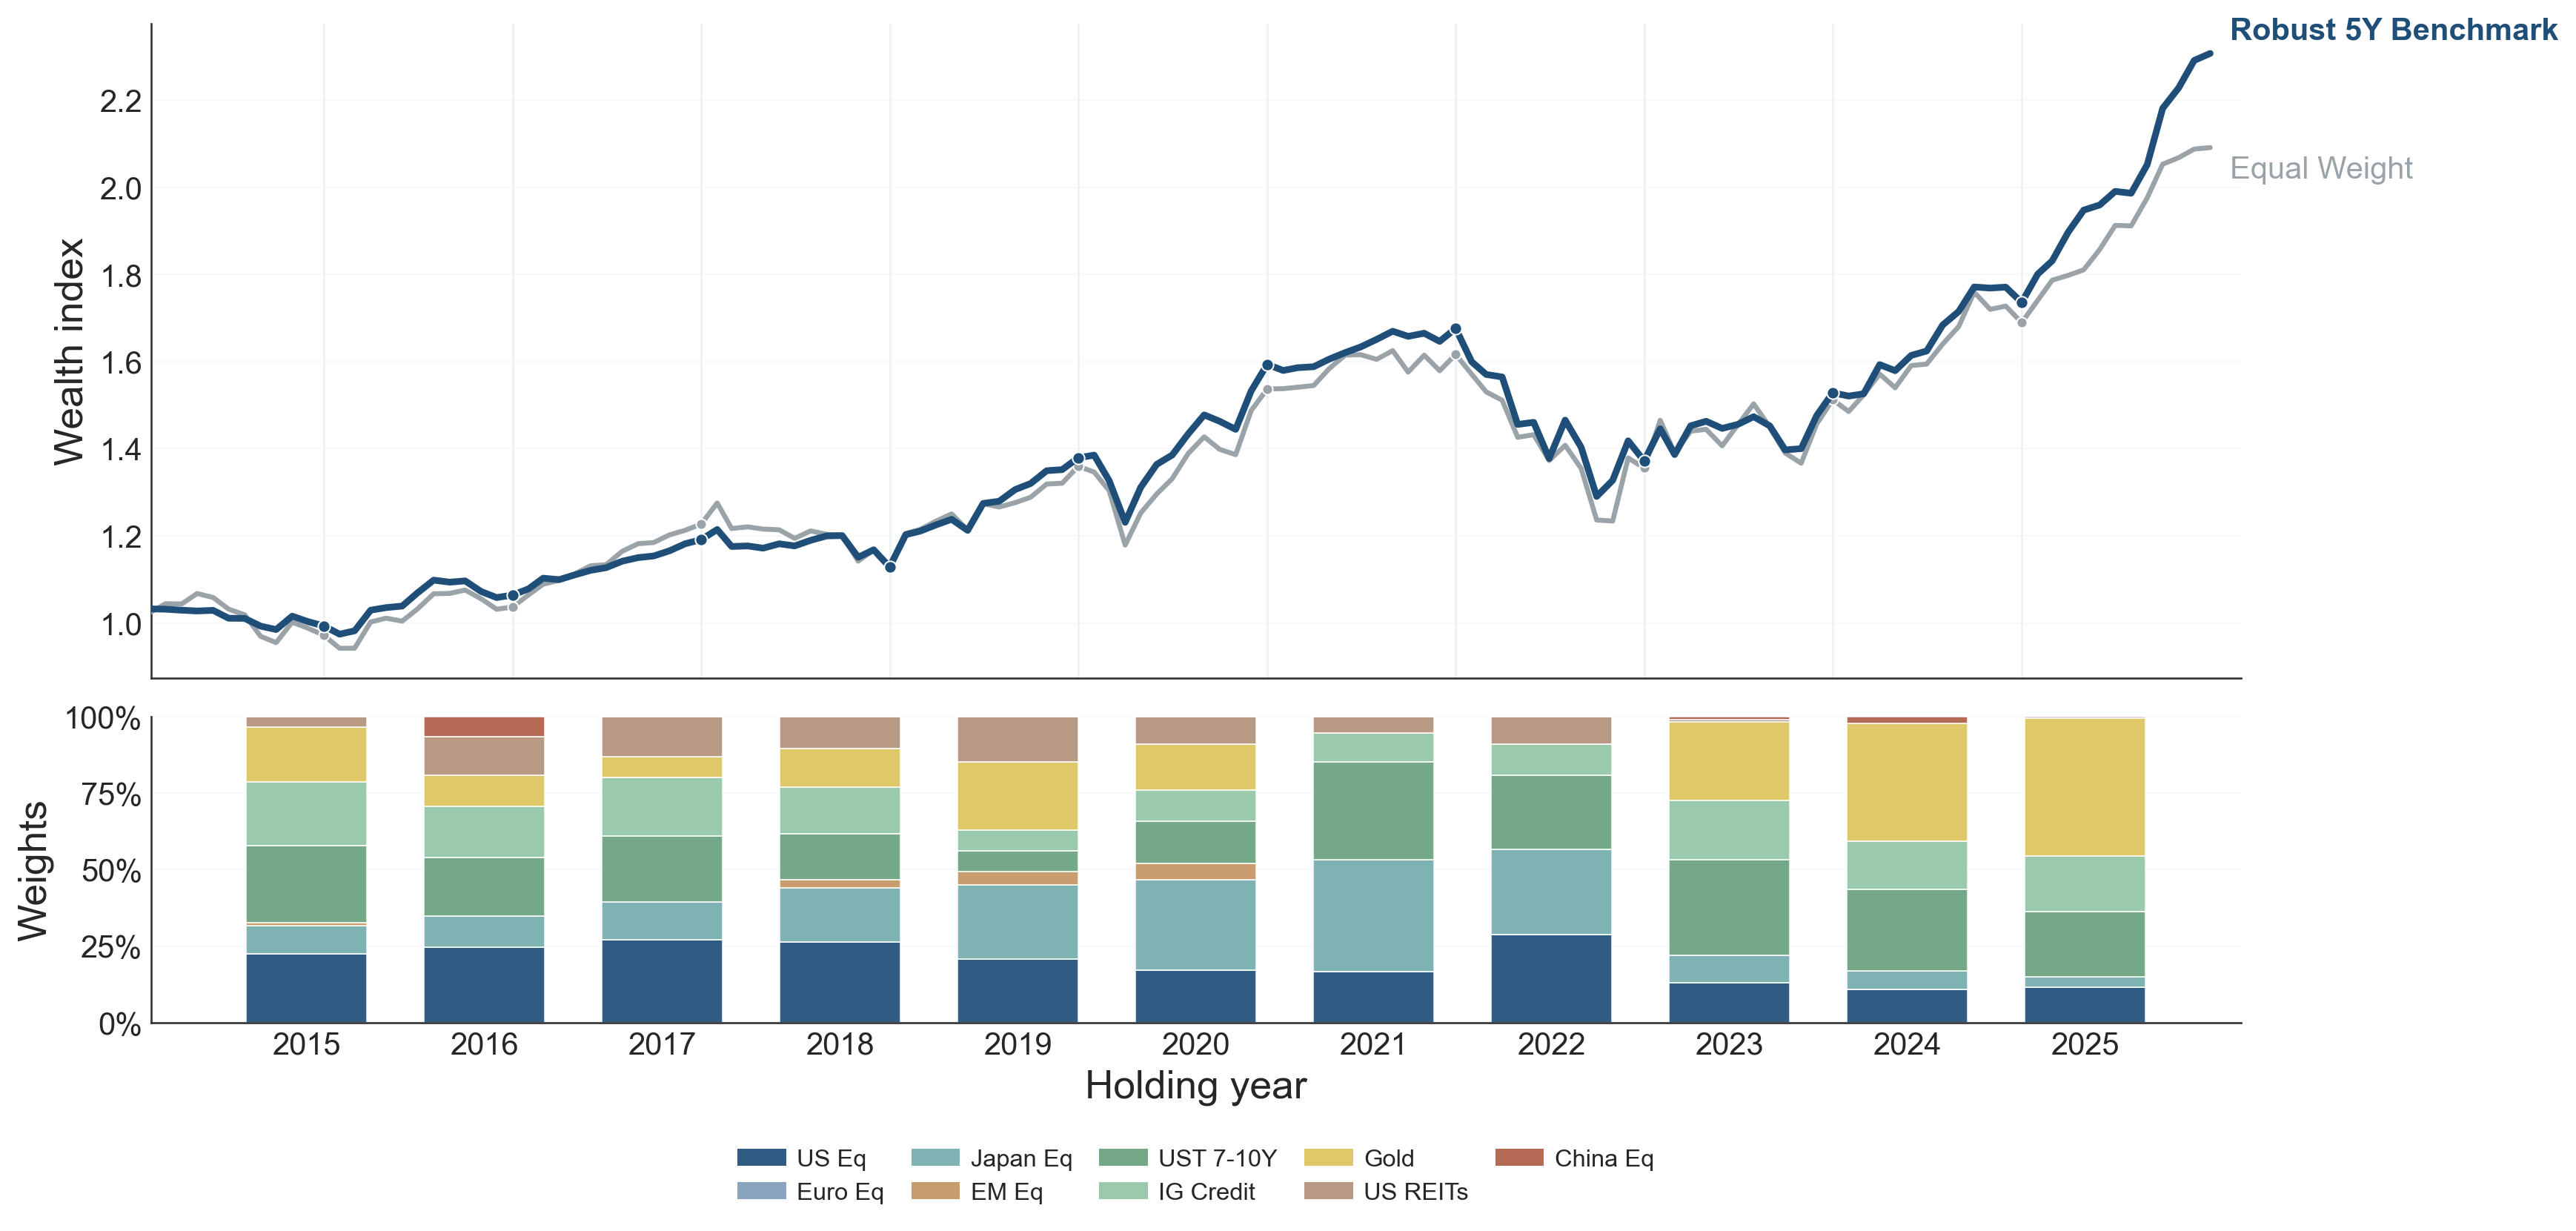
\includegraphics[width=\linewidth,height=0.72\textheight,keepaspectratio]{portfolio_wealth_path_best_60.pdf}
\end{columns}
\end{frame}

\begin{frame}{From Prediction to Portfolio}
\begin{columns}[T,totalwidth=\textwidth]
\column{0.5\textwidth}
\centering
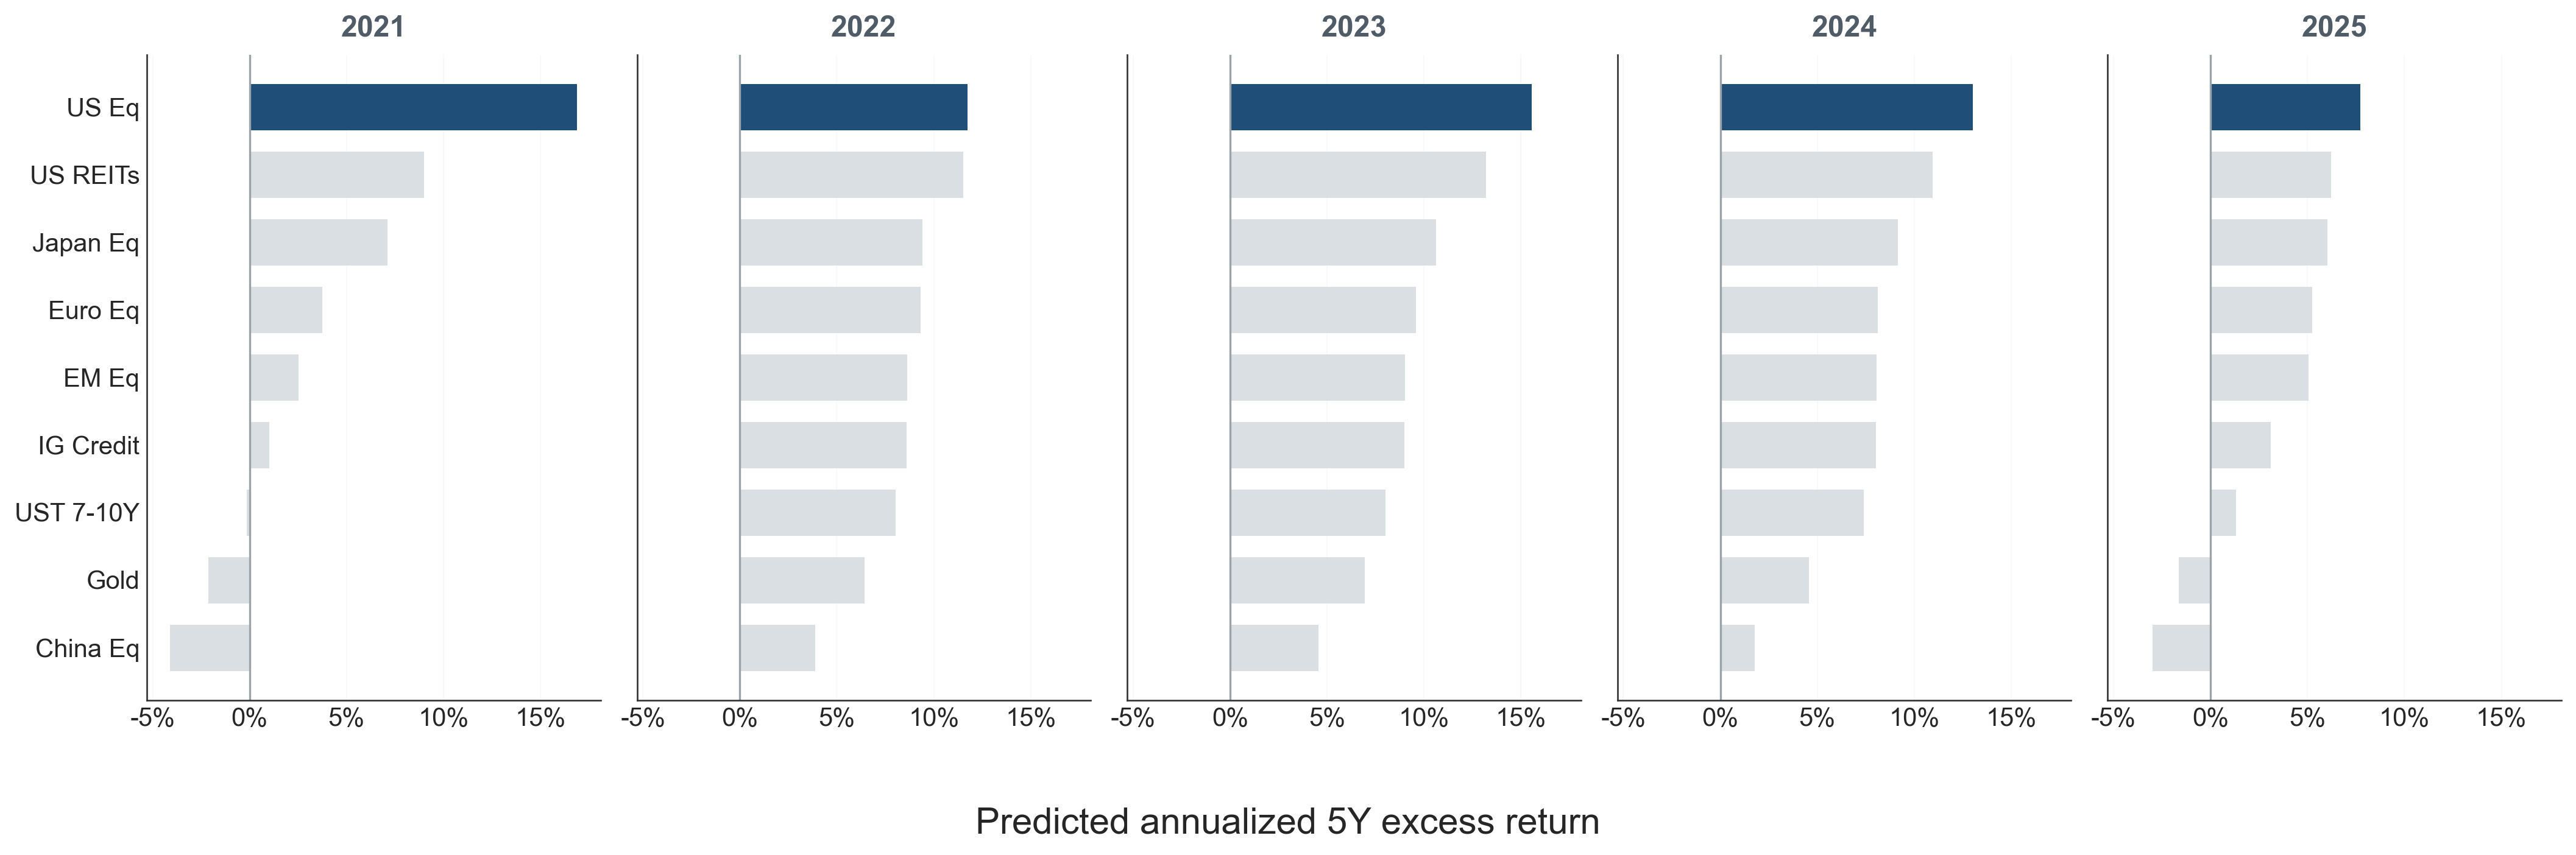
\includegraphics[width=\linewidth,height=0.65\textheight,keepaspectratio]{recent_prediction_snapshot_5y.pdf}
\vspace{0.3em}

{\small Forward-looking 5Y sleeve return views}

\column{0.5\textwidth}
\centering
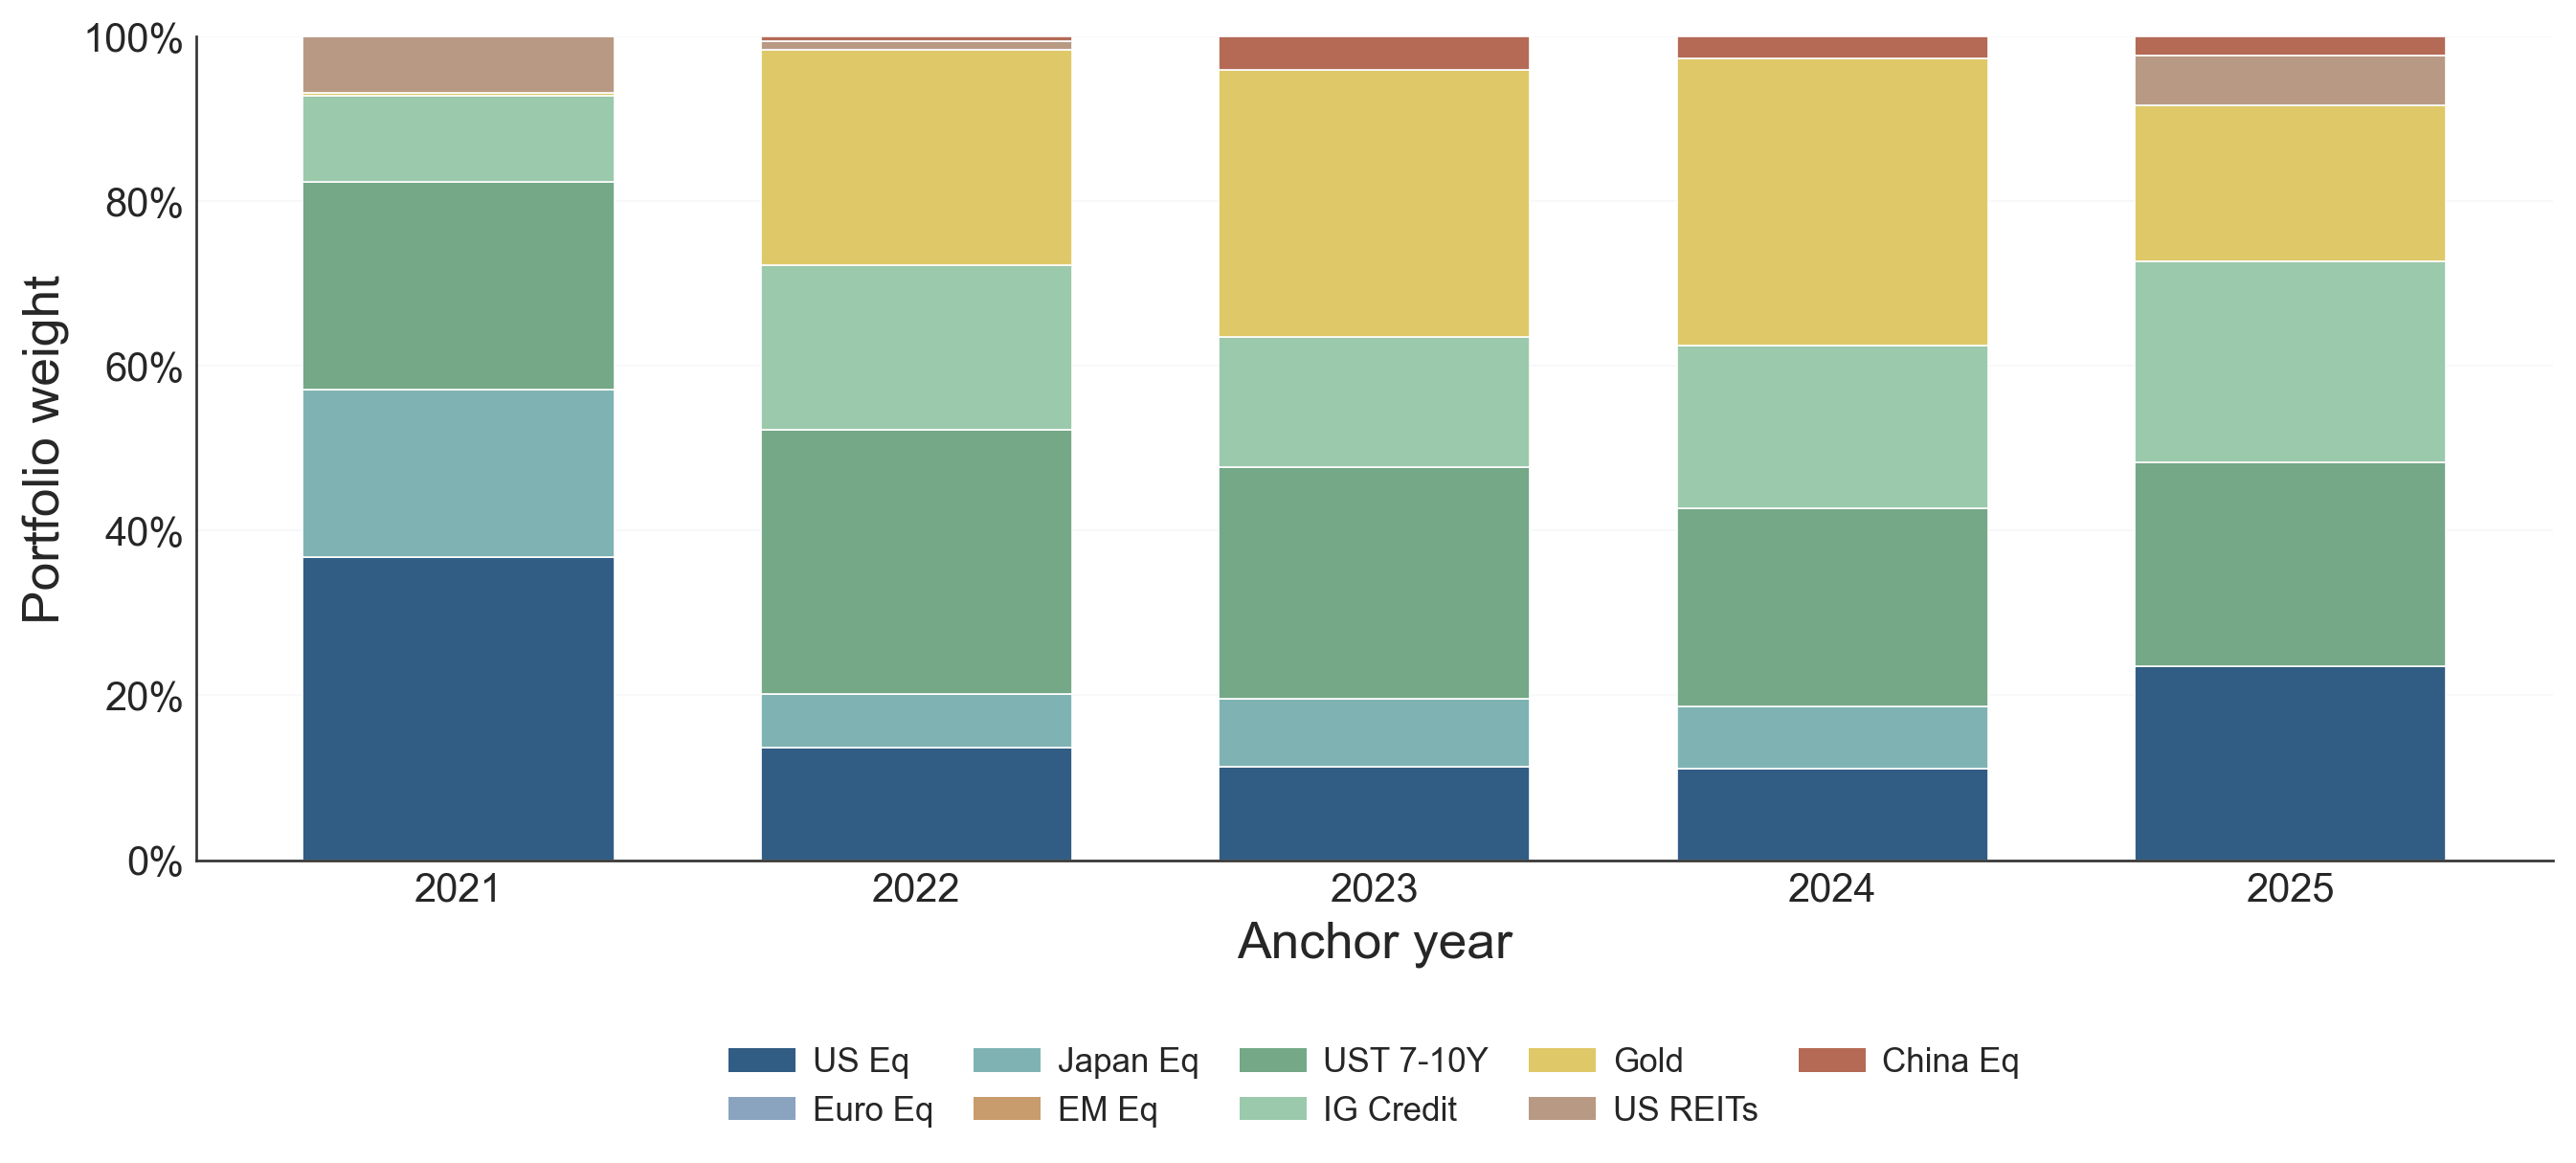
\includegraphics[width=\linewidth,height=0.65\textheight,keepaspectratio]{recent_portfolio_snapshot_5y.pdf}
\vspace{0.3em}

{\small Model-implied 5Y portfolio allocations}
\end{columns}
\vspace{0.4em}
{\small\color{muted}The bridge to scenario generation is that the model produces full portfolio decisions, not only return forecasts.}
\end{frame}

\begin{frame}{How Scenario Generation Works}
\begin{itemize}
  \item Start from a real month-end market state.
  \item Move a compact macro-financial state in plausible directions.
  \item Hold the richer cross-asset context fixed at the anchor date.
  \item Re-evaluate the benchmark under the new state.
  \item Compare baseline vs scenario in terms of:
  \begin{itemize}
    \item expected long-run return
    \item concentration
    \item full 9-sleeve allocation
  \end{itemize}
\end{itemize}
\vspace{0.7em}
\textbf{Scenario levers}
\begin{itemize}
  \item inflation, unemployment, short rates, long rates
  \item dollar strength, market volatility, real rates, credit spreads, oil
  \item across the US, Euro Area, and Japan
\end{itemize}
\end{frame}

\begin{frame}{How We Label Regimes}
\begin{columns}[T,totalwidth=\textwidth]
\column{0.5\textwidth}
\textbf{Internal dimensions}
\begin{itemize}
  \item Growth
  \item Inflation
  \item Stress
  \item Rates / conditions
\end{itemize}

\vspace{0.5em}
\textbf{External anchors}
\begin{itemize}
  \item Chicago Fed NFCI
  \item NBER recession overlay
\end{itemize}

\column{0.5\textwidth}
\textbf{Regime labels}
\begin{itemize}
  \item Soft landing
  \item Higher-for-longer
  \item Risk-on reflation
  \item High-stress defensive
  \item Disinflationary slowdown
  \item Mixed mid-cycle
\end{itemize}
\vspace{0.7em}
{\small\color{muted}This is a transparent macro scorecard for interpretation, not a black-box hidden-state model.}
\end{columns}
\end{frame}

\begin{frame}{The Four Main Questions}
\begin{enumerate}
  \item What does a soft-landing regime look like for the benchmark?
  \item What does a higher-for-longer regime look like for the benchmark?
  \item What regime makes gold more attractive inside the benchmark?
  \item What regime improves return without making the benchmark much more concentrated?
\end{enumerate}
\vspace{1em}
\textbf{Three representative scenario cases}
\begin{itemize}
  \item Upside case: return improves without destabilizing the portfolio
  \item Breadth case: diversification improves, but not for free
  \item Adverse case: tighter conditions weaken the outlook and keep the benchmark more defensive
\end{itemize}
\end{frame}

\begin{frame}{What Kind of Scenarios Matter for the Benchmark?}
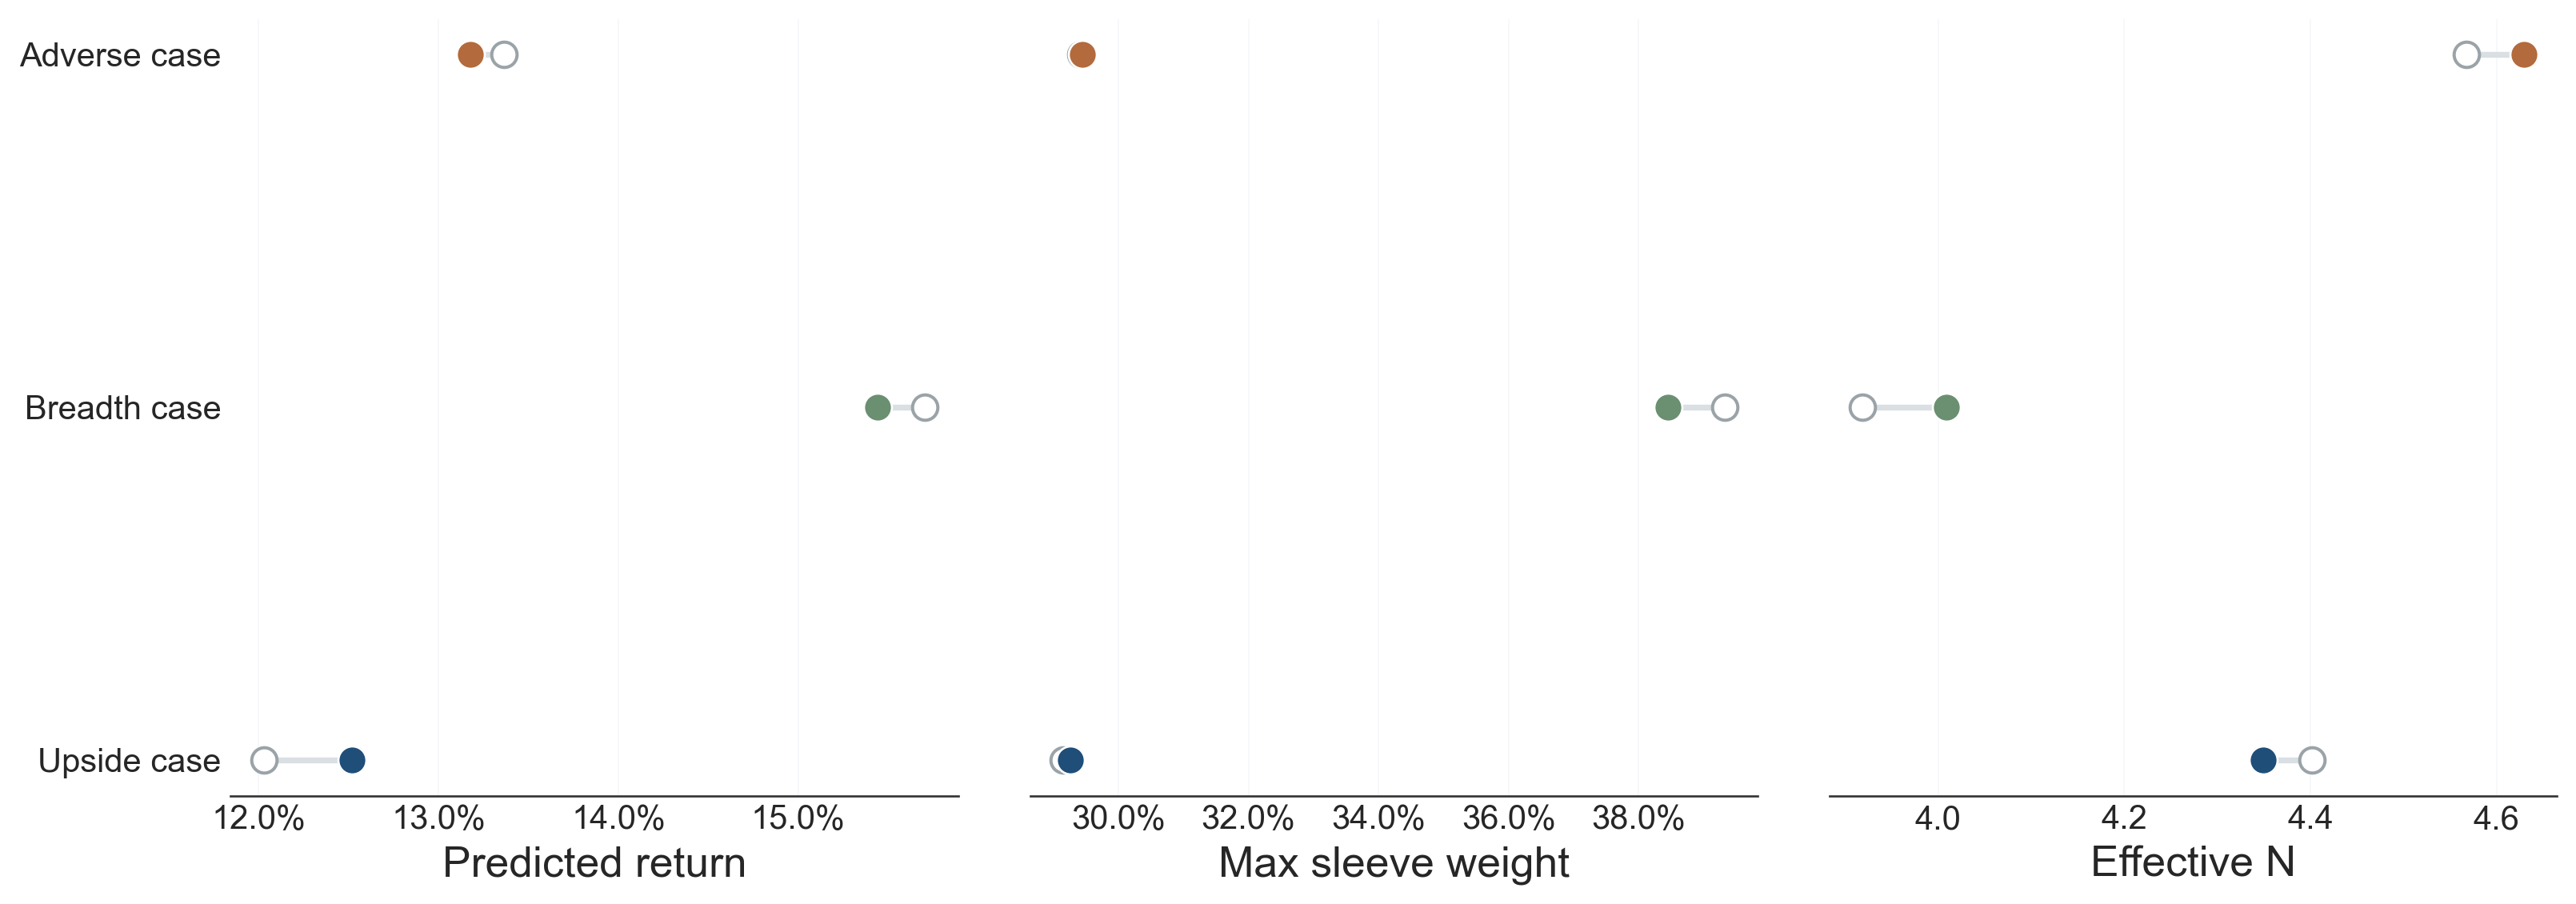
\includegraphics[width=\linewidth,height=0.82\textheight,keepaspectratio]{scenario_case_benchmark_story_v3.pdf}
\end{frame}

\begin{frame}{How the Portfolio Changes Under the Scenario}
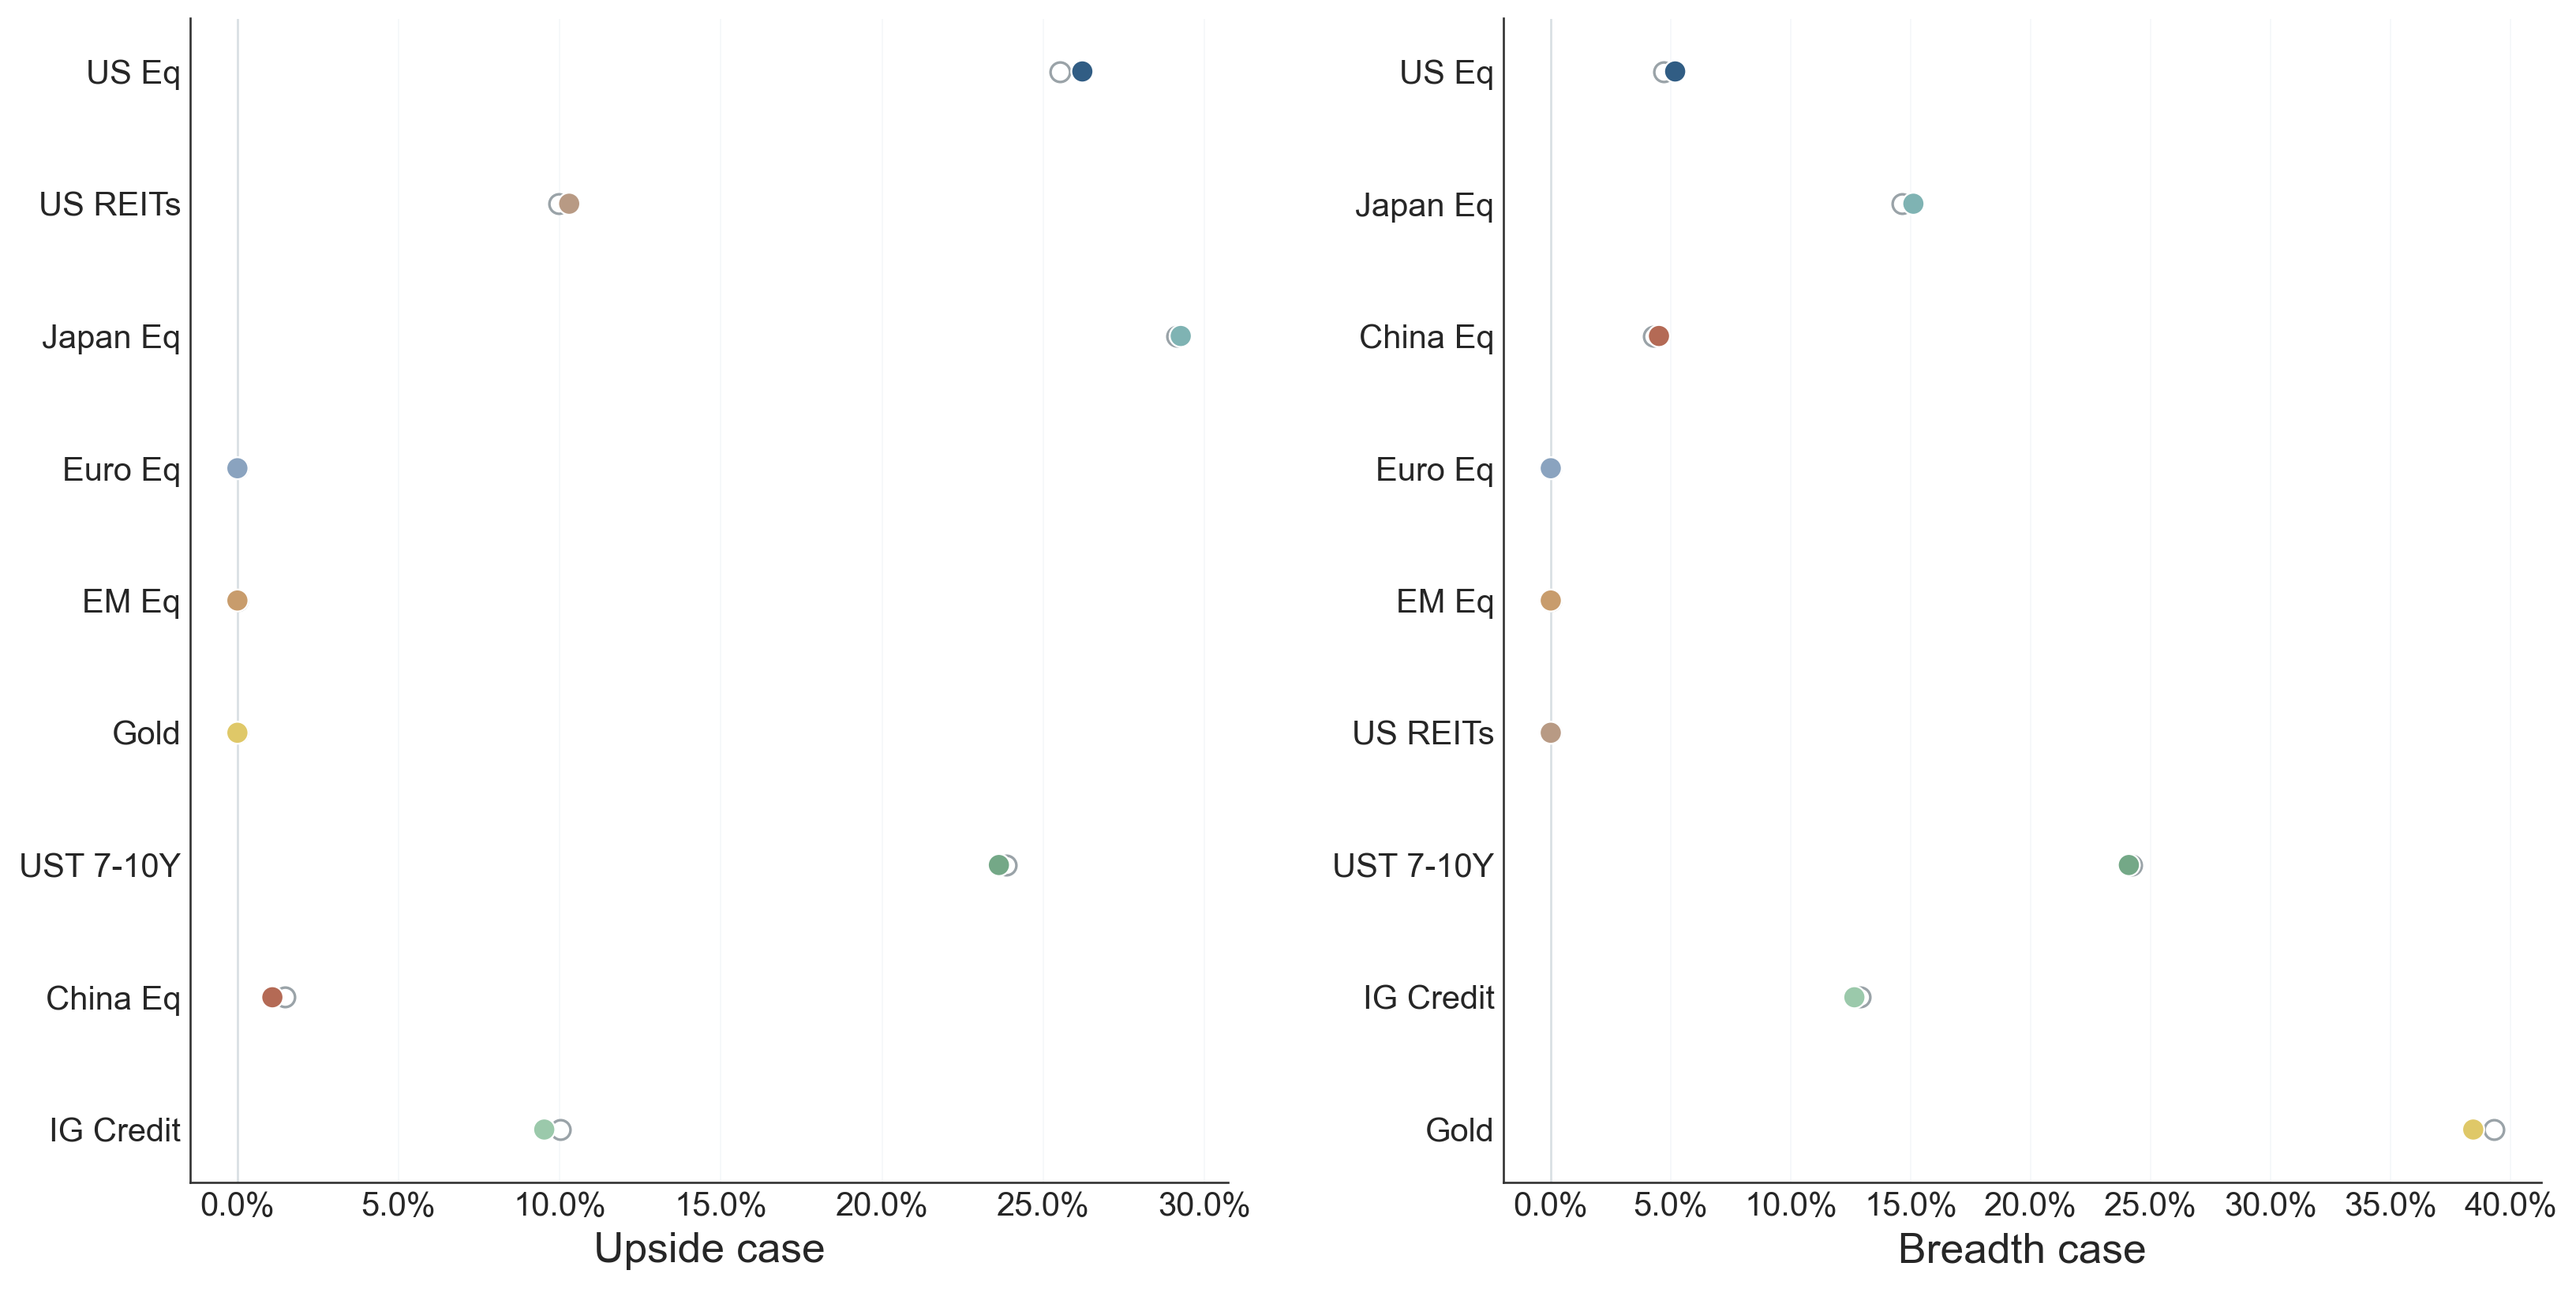
\includegraphics[width=\linewidth,height=0.82\textheight,keepaspectratio]{scenario_case_allocation_change_v3.pdf}
\end{frame}

\begin{frame}{Macro Fingerprints Behind the Cases}
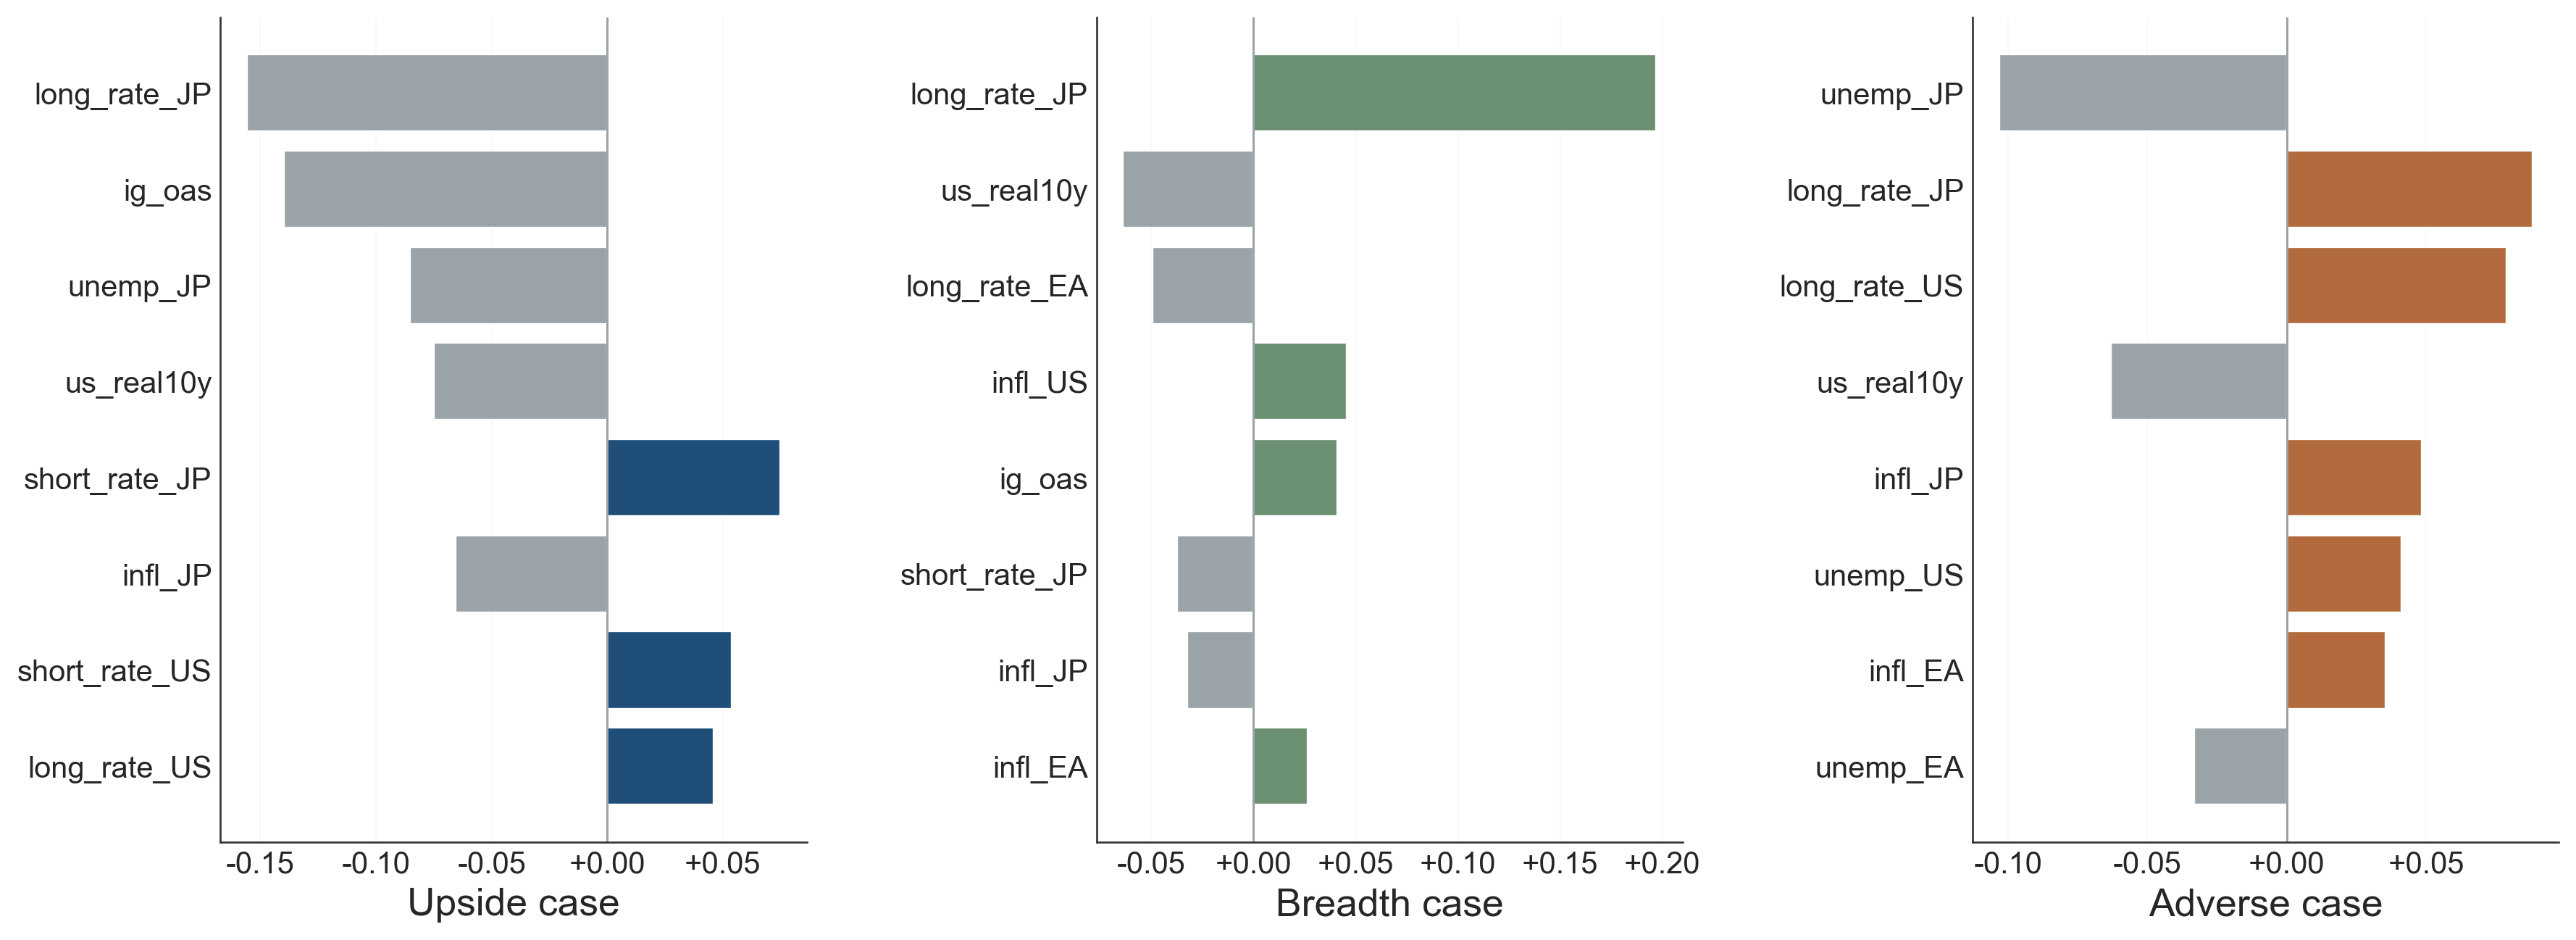
\includegraphics[width=\linewidth,height=0.82\textheight,keepaspectratio]{scenario_case_macro_fingerprint_v3.pdf}
\end{frame}

\begin{frame}{Final Takeaway}
\begin{itemize}
  \item The framework connects long-run capital-market views to portfolio allocation decisions.
  \item The benchmark is credible enough to interpret at the portfolio level.
  \item The scenario layer identifies plausible macro-financial states that support stronger, weaker, broader, or more defensive outcomes.
  \item The end product is an interpretable strategic allocation scenario engine.
\end{itemize}
\end{frame}

\end{document}
